\documentclass[11pt,a4paper]{article}
\usepackage[T1]{fontenc}
\usepackage[utf8]{inputenc}
\usepackage{mathptmx}
\usepackage[margin=21mm,top=20mm,bottom=20mm,headheight=14pt,headsep=7mm]{geometry}
\usepackage{microtype}
\usepackage{array,tabularx,booktabs}
\usepackage{titlesec}
\usepackage{caption}
\usepackage{fancyhdr,lastpage}
\usepackage{graphicx}
\graphicspath{{source/}}
\usepackage{xurl}
\usepackage[hidelinks]{hyperref}

\hypersetup{
  pdftitle={DepthScope Data Milestone Report},
  pdfauthor={Igor Kołodziej, Adam Kaniasty, Mateusz Iwaniuk, Hubert Kowalski},
  pdfsubject={Data acquisition and pre-processing}
}
\urlstyle{same}

\setlength{\parindent}{0pt}
\setlength{\parskip}{5pt}
\linespread{1.04}
\titleformat{\section}{\large\bfseries}{\thesection}{0.65em}{}
\titlespacing*{\section}{0pt}{11pt}{5pt}
\titleformat{\subsection}{\normalsize\bfseries}{\thesubsection}{0.65em}{}
\titlespacing*{\subsection}{0pt}{7pt}{3pt}
\captionsetup{font=small,labelfont=bf,labelsep=period,skip=5pt}
\renewcommand{\arraystretch}{1.13}
\newcolumntype{L}[1]{>{\raggedright\arraybackslash}p{#1}}
\newcolumntype{Y}{>{\raggedright\arraybackslash}X}

\pagestyle{fancy}
\fancyhf{}
\fancyhead[L]{\small DepthScope}
\fancyhead[R]{\small Data milestone}
\fancyfoot[C]{\small\thepage\ of \pageref*{LastPage}}
\renewcommand{\headrulewidth}{0.35pt}
\renewcommand{\footrulewidth}{0pt}
\fancypagestyle{plain}{%
  \fancyhf{}%
  \fancyfoot[C]{\small\thepage\ of \pageref*{LastPage}}%
  \renewcommand{\headrulewidth}{0pt}%
}

\begin{document}
\thispagestyle{plain}

\begin{center}
{\fontsize{23}{26}\selectfont\bfseries DepthScope}\par
\vspace{5pt}
{\fontsize{15}{18}\selectfont Data acquisition and pre-processing\\Data milestone report}\par
\vspace{6pt}
{\small Igor Kołodziej \quad Adam Kaniasty \quad Mateusz Iwaniuk \quad Hubert Kowalski}\par
\vspace{6pt}
{\small 21 November 2026\par}
\end{center}
\vspace{2pt}

\section{Updates to the PM1 assumptions}
DepthScope will compare visible BTC/USD and ETH/USD liquidity on Coinbase Exchange and Kraken and later forecast liquidity 60 seconds ahead. This checkpoint covers acquisition, source validation, storage and archiving.

The native component uses C17 instead of C++ to keep source-book validation in a small fixed-point library. Python hosts the library through \texttt{ctypes} and handles network connections and service orchestration. A second processor thread batches raw messages into ClickHouse every three seconds or 5,000 messages for data-quality queries. The complete Parquet archive will support later historical reprocessing. All runtime services run in Docker Compose on one host with persistent volumes.

\section{Conceptual data model}
\begin{table}[h!]
\centering\small
\begin{tabularx}{\textwidth}{@{}L{35mm}Y@{}}
\toprule
\textbf{Entity} & \textbf{Key information and role}\\
\midrule
Venue / instrument & Venue, base asset and USD quote identify one of four source books.\\
Raw event & Original message, receipt timestamps, venue and event kind. The Kafka offset defines its stream position.\\
Book state & Current ordered source levels and validation state, maintained in memory.\\
Archive batch & Parquet objects and a manifest with offset and receipt-time bounds.\\
Acquisition record & Venue, asset, second, source status, book levels and instrument increments.\\
Acquisition stream & Live acquisition records, identified by venue, asset and receipt-time second.\\
Fee row & Venue, effective date, maker/taker rates, observed date, tier and source URL.\\
\bottomrule
\end{tabularx}
\end{table}

A venue lists instruments. Each instrument produces many raw events and acquisition records. Raw events are grouped into archive batches, whose manifests retain stream offsets and receipt-time bounds. Each venue has dated fee rows. On processor startup, fresh source snapshots establish the current book state; processor checkpoints and a historical replay reader are planned for later work.

Raw messages are retained in full. Normalized one-second records provide a view of validated book state, while the raw stream preserves every captured update and trade.

\newpage
\section{Description of the data sets}
\subsection{Market streams and public metadata}
Both venues provide public JSON streams for BTC and ETH quoted in USD. Coinbase Exchange uses \texttt{level2\_batch}, \texttt{matches}, \texttt{heartbeat} and \texttt{status}. Kraken Spot WebSocket v2 uses \texttt{book} at depth 1,000, \texttt{trade} and \texttt{instrument}, together with feed-control messages.

\begin{table}[h!]
\centering\small
\begin{tabularx}{\textwidth}{@{}L{27mm}YY@{}}
\toprule
\textbf{Record category} & \textbf{Available fields} & \textbf{Format and arrival}\\
\midrule
Book snapshot / update & Price, absolute quantity and side; symbol, exchange time and Kraken CRC32 where supplied. & JSON. Initial snapshot followed by incremental changes. Coinbase book changes are batched every 50 ms when present; Kraken is event driven.\\
Trade & Trade ID, price, quantity, timestamp and source-side information in the original payload. & JSON, event driven. Several trades can share one message.\\
Instrument / feed status & Market status, price and quantity increments, heartbeat and connection information. & JSON snapshots, updates and control messages.\\
\bottomrule
\end{tabularx}
\end{table}

\subsection{Measured inflow and coverage}
The measured receipt-time interval is 21 November 2026, 20:43:46--20:45:45 UTC, covering 120 seconds. Counts combine BTC and ETH and all subscribed channels for each venue.

\begin{table}[h!]
\centering\small
\begin{tabularx}{\textwidth}{@{}Yrrr@{}}
\toprule
\textbf{Venue} & \textbf{Messages} & \textbf{Mean msg/s} & \textbf{Payload kB/s}\\
\midrule
Coinbase Exchange & 4,538 & 37.82 & 24.6\\
Kraken Spot v2 & 20,547 & 171.22 & 33.1\\
\bottomrule
\end{tabularx}
\end{table}

One message can contain several level changes or trades. Byte rates exclude transport and storage overhead. Each of the four books produced 120 unique, valid acquisition records, giving 480 records in total. History is available from the first captured usable snapshot. The short sample establishes observed operation rather than long-run capacity. Kraken CRC32 checks cover the best ten levels. Internal trade-ID gaps and a missing initial snapshot need stronger detection before later trade-flow analytics.

\subsection{Fee schedule batch input}
The dated CSV contains two selected standard entry-tier fee rows observed on 21 November 2026. It retains venue, effective UTC, maker/taker basis points, observed UTC, tier and source URL. The effective date is the observation-date scenario boundary. Account tiers and pair discounts can differ. Source URLs are retained directly in the input file.

\section{Data acquisition, transformation and storage}
Python collectors subscribe to the public channels without trading credentials, timestamp each received message and publish it to Kafka. Reconnection uses capped backoff. Source rates vary with market activity, so the collector reports measured message rates and downstream lag.

Book prices and quantities are decoded as decimals and stored as exact $10^{-8}$ units in C. Updates replace absolute level quantities, zero removes a level, and trades do not decrement the book again. Validation rejects crossed or locked books, verifies Kraken checksums and tracks Coinbase heartbeat consistency. Unavailable book state is flagged in acquisition records. Raw events are batched into ClickHouse and archived as Zstandard-compressed Parquet, partitioned by venue, asset, date and hour.

\newpage
\section{System architecture}
\begin{figure}[h!]
\centering
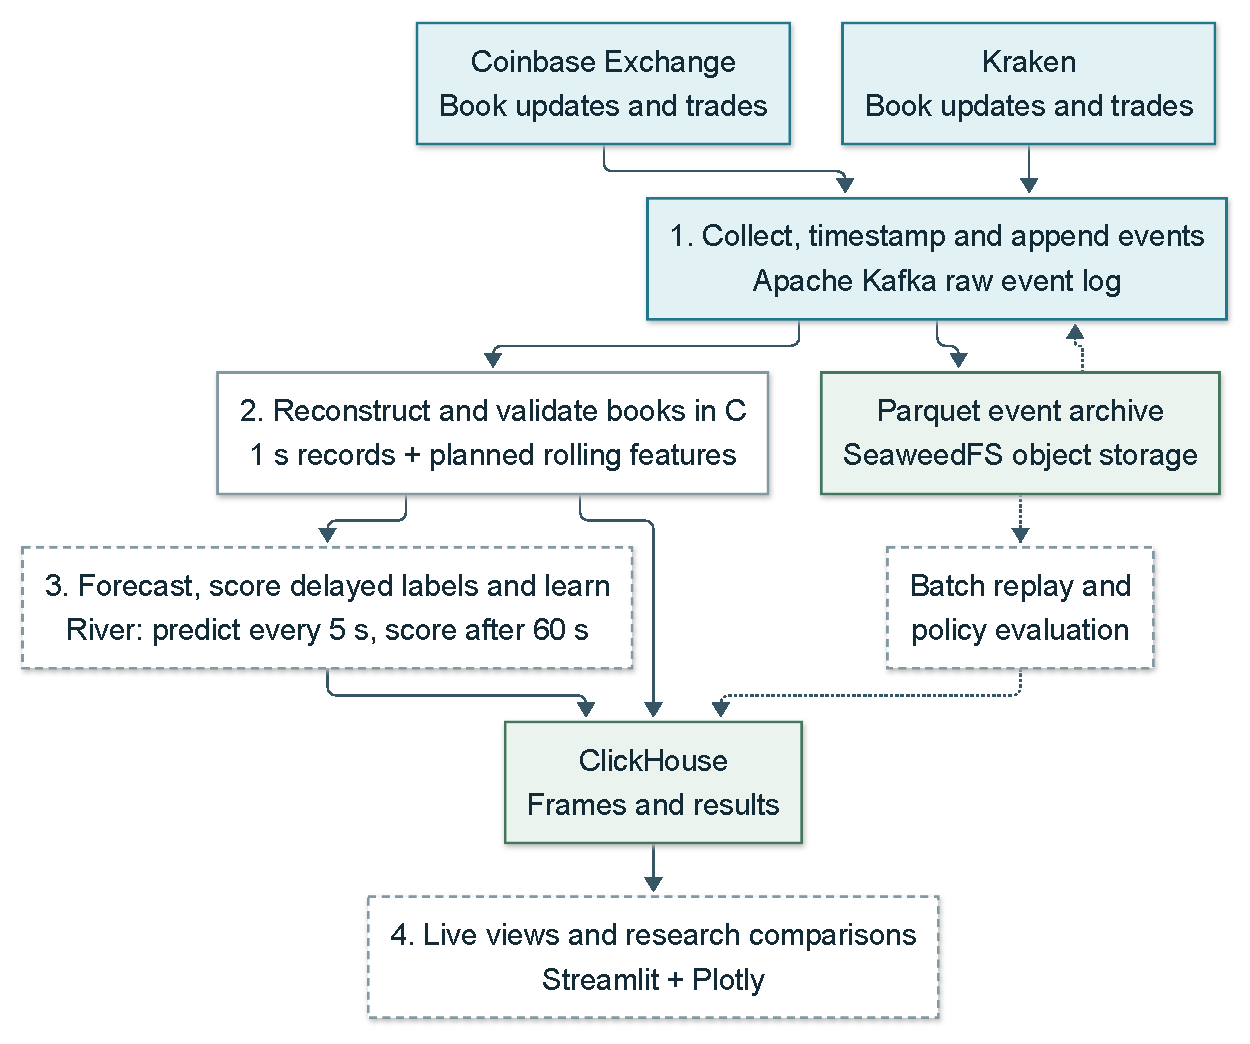
\includegraphics[width=\linewidth,height=124mm,keepaspectratio]{system-architecture.pdf}
\caption{DepthScope Kappa architecture, adapted from the project proposal. Dashed boxes mark planned modules. Dashed arrows mark replay via Kafka and batch evaluation.}
\end{figure}

Python collectors timestamp the WebSocket messages and append them to Kafka. The processor keeps the current books in C and publishes validated levels and feed status every second. A separate thread writes raw events to ClickHouse, and a Kafka consumer stores the one-second book records there.

The archiver writes raw messages and offset manifests to SeaweedFS for later replay through the same validation code. The Python fee loader selects rates by effective date for later batch evaluation. The acquisition and storage services run in Docker Compose.

\section{Planned analytical approach and presentation}
The planned regression task is to predict visible USD liquidity 60 seconds ahead for each venue, asset and trade side. The target will sum asks up to 0.10\% above the future midpoint for buying, or bids down to 0.10\% below it for selling.

Book and trade streams will supply planned depth, spread, imbalance, trade-flow and volatility features, with instrument metadata used for validation. Online linear regression and an adaptive random forest are candidates, compared with persistence and EWMA baselines. Stream processing will generate the features and forecasts. Archived streams will support chronological evaluation and comparisons between venue-specific and combined inputs. The fee CSV will support later execution-cost experiments.

The proposed presentation layer is a Streamlit application with Plotly charts. It will show per-venue liquidity, future forecasts and observed outcomes, alongside acquisition status and data coverage. Users will select an asset and trade side to inspect the relevant market views.
\end{document}
